\chapter{Nonlinear Dimensionality Reduction}

Although PCA has presented promising results in the previous section, hence its great popularity in dimensionality reduction problems, there are many examples in which PCA will fail in its task. Consider the example bellow:

\begin{figure}[H]
	\centering
	\captionsetup{justification=centering}

	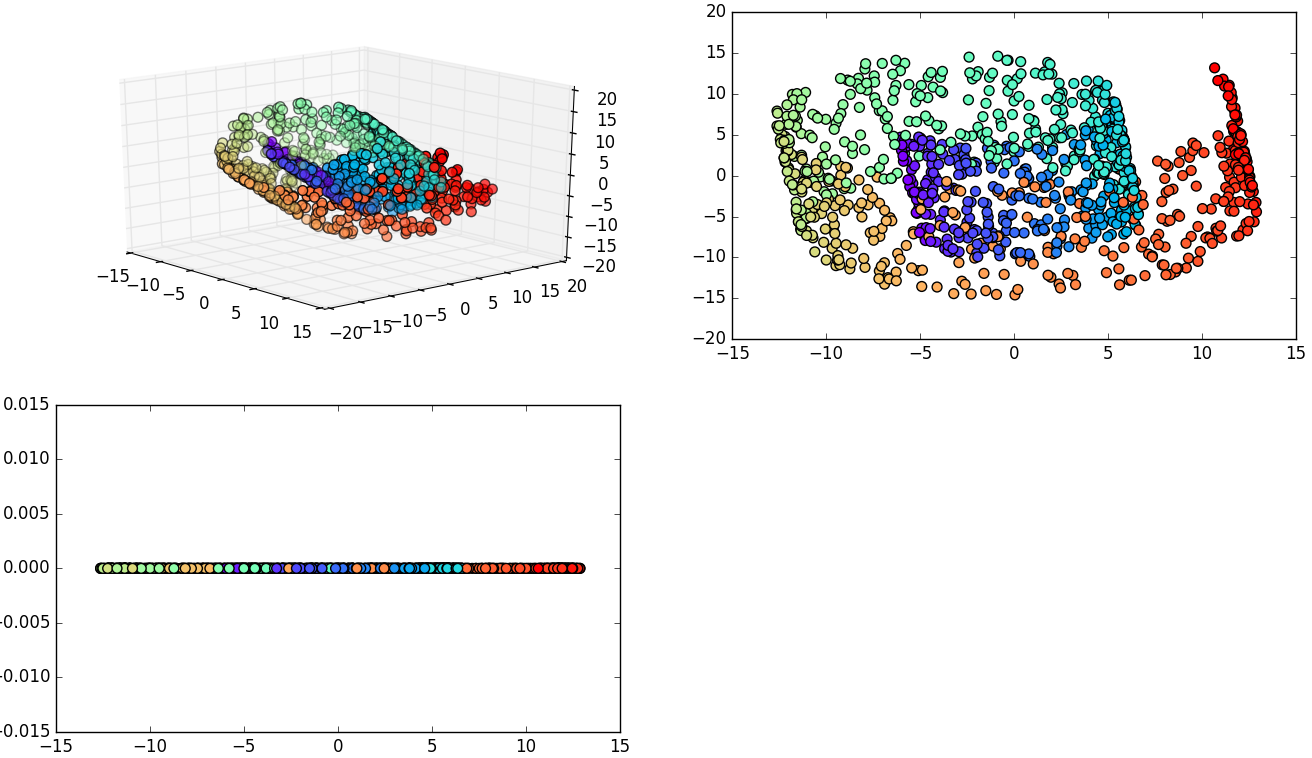
\includegraphics[width=\linewidth]{experiments/pca_swiss}
	\caption{The \textbf{Swiss-roll manifold} and its reductions to 3, 2 and 1 dimensions, respectively, using the PCA algorithm.}
	\label{fig:swiss_pca}
\end{figure}21

Looking at figure \ref{fig:swiss_pca} (specially in the last reduction, to a single dimension), it becomes clear that PCA has a big draw back: it assumes that the data lies on a liner subspace \cite{cay2005} and, therefore, applying linear transformations to it will rotate and scale it, without distort the original data structure. When this assumption does not hold, PCA will incorrectly extract the underlying structure, possibly mixing very dissimilar samples.

The table bellow describes a regression attempt over the data sets illustrated in figure \ref{fig:swiss_pca}, were the feature being predicted is the contiguous value represented by the vertexes' colors:

\begin{table}[H]
	\centering
	\begin{tabular}{|c|c|c|c|c|}
		\hline
		& \textbf{Original data} & \textbf{Reduc. ($\mathbb{R}^3$)} & \textbf{Reduc. ($\mathbb{R}^2$)} & \textbf{Reduc. ($\mathbb{R}^1$)} \\\hline
		\textbf{Accuracy} & 1. & 1. & .68 & .54 \\\hline
		\textbf{GS time}  & 10.98 s & 10.48 s & 5.20 s & 2.59 s \\\hline
		\textbf{Reduc. time} & - & 0.038 s & 0.038 s & 0.035 s \\\hline
		\textbf{Stress} & - & 0 & .2788 & .5271 \\\hline
		\textbf{Data size} & 23.44 KB & 23.44 KB & 15.62 KB  & 7.81 KB \\\hline
	\end{tabular}

	\captionsetup{justification=centering}
	\caption{Regression accuracy and reduction performance for the Swiss-roll data set.}
\end{table}

Clearly, linear dimensionality reduction techniques are not adequate to reduce the Swiss-roll. In fact, it is not adequate to reduce any data set lying on a nonlinear manifold.

\section{The ISOMAP Algorithm}

Firstly suggested by Tenenbaum, de Silva and Langfor, \textbf{Isometric Feature Mapping} (or ISOMAP) assumes that the data lies near a smooth manifold. If the assumption is reasonable, it is be possible to explore concepts such as neighborhood and local linearity to map the manifold to a linear structure before reducing it with a linear algorithm.

In this section we will discuss the ISOMAP algorithm and its inner workings. We will then proceed to formalize it. Finally, empirical tests results achieved during the project will be shown.

\subsection{Study of the ISOMAP Algorithm}
\label{sec:studying_ISOMAP}

As the original data set might be folded, twisted or curved, \cite{ten2000} we must first find a suitable linear representation for it.

Let $S$ be our original data set, as illustrated in figure \ref{fig:mani_s}.

\begin{figure}[H]
	\centering
	\captionsetup{justification=centering}
	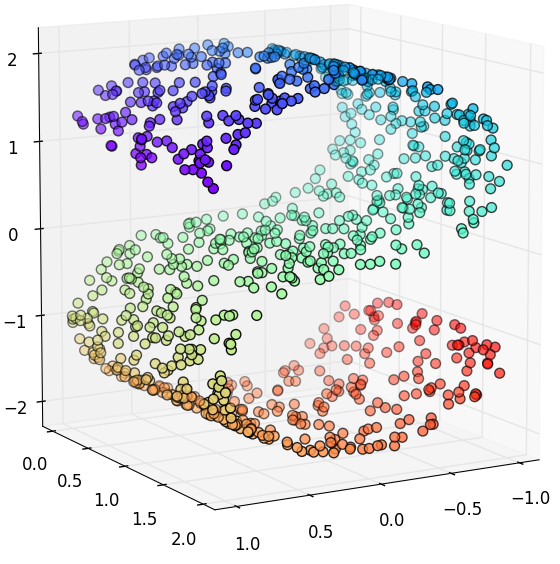
\includegraphics[width=.5\linewidth]{datasets/s}
	\caption{The data set $S$, consisting of $1000$ samples and $3$ features.}
	\label{fig:mani_s}
\end{figure}

Additionally, consider the symmetric undirected weighted graph $G=(V, E)$ and $w \colon E \to \mathbb{R} \mid w(x, y) = \delta_{xy}$, where $\delta_{xy}$ is the euclidean distance between the samples $x$ and $y$ in $S$. That is,
$$\delta_{xy} = \sqrt{\sum_{i} (x_i - y_i)^2}, \forall (x, y) \in S\times S \mid x\ne y$$

Now that only distances were kept, an infinite number of n-dimensional embeddings can be found with \textbf{MDS}, as every solution can be transposed, rotated or reflected. This does not fix the non-linearity of the data, though, as the original distances strictly constraint the samples to their original pattern. In order to achieve this, \textbf{Nearest neighbor search} can be performed over $G$, resulting in the graph $H$. Nearest-neighbor search will preserve edges connecting closer samples, hence preserving local (linear) distances, but erase edges connecting samples which are far from each other (non necessarily linear). Obviously, the search parameters ($K$ or $\epsilon$) must be carefully chosen to limit the connectivity of the vertices to a small (linear) neighborhood while maintaining the graph completely connected. Ideally, $H$ will be a \textbf{mesh graph}.

\begin{figure}[H]
	\centering
	\captionsetup{justification=centering}
	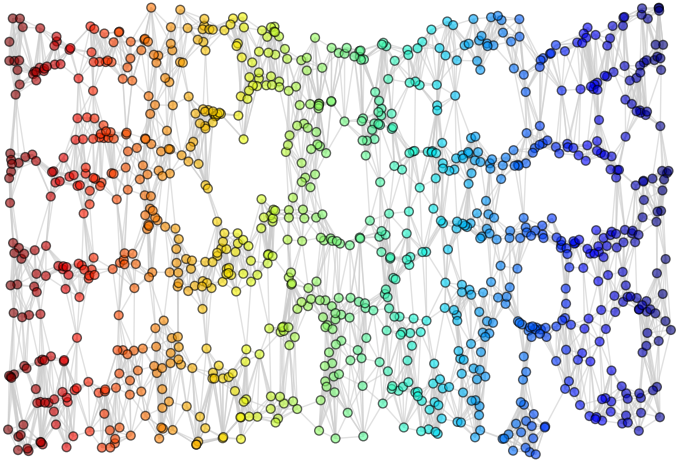
\includegraphics[width=.5\linewidth]{studying_isomap/neighbors}
	\caption{The graph $H$.}
	\label{fig:mani_s_graph_h}
\end{figure}

At this moment, not all distances in $H$ are defined. This can be easily handled, though, by performing the \textbf{Floyd-Warshall} algorithm over $H$. Alternatively, $M$ can be achieved by performing \textbf{Dijkstra's algorithm} for all nodes and joining all shortest-path trees found.

Finally, $M$ is a euclidean graph which roughly lies on a linear subspace. Furthermore, the adjacency matrix associated to $M$ contains not the distance induced by the $L_2$ norm, but the geodesic pairwise distances. \cite{gho2006} The \textbf{MDS} method can now be used to construct a representation in sub-spaces of the $\mathbb{R}^n$. $S$, specifically, can be reduced to the $\mathbb{R}^2$ or $\mathbb{R}$:

\begin{figure}[H]
    \begin{subfigure}{.5\linewidth}
		\centering
		\captionsetup{justification=centering}
		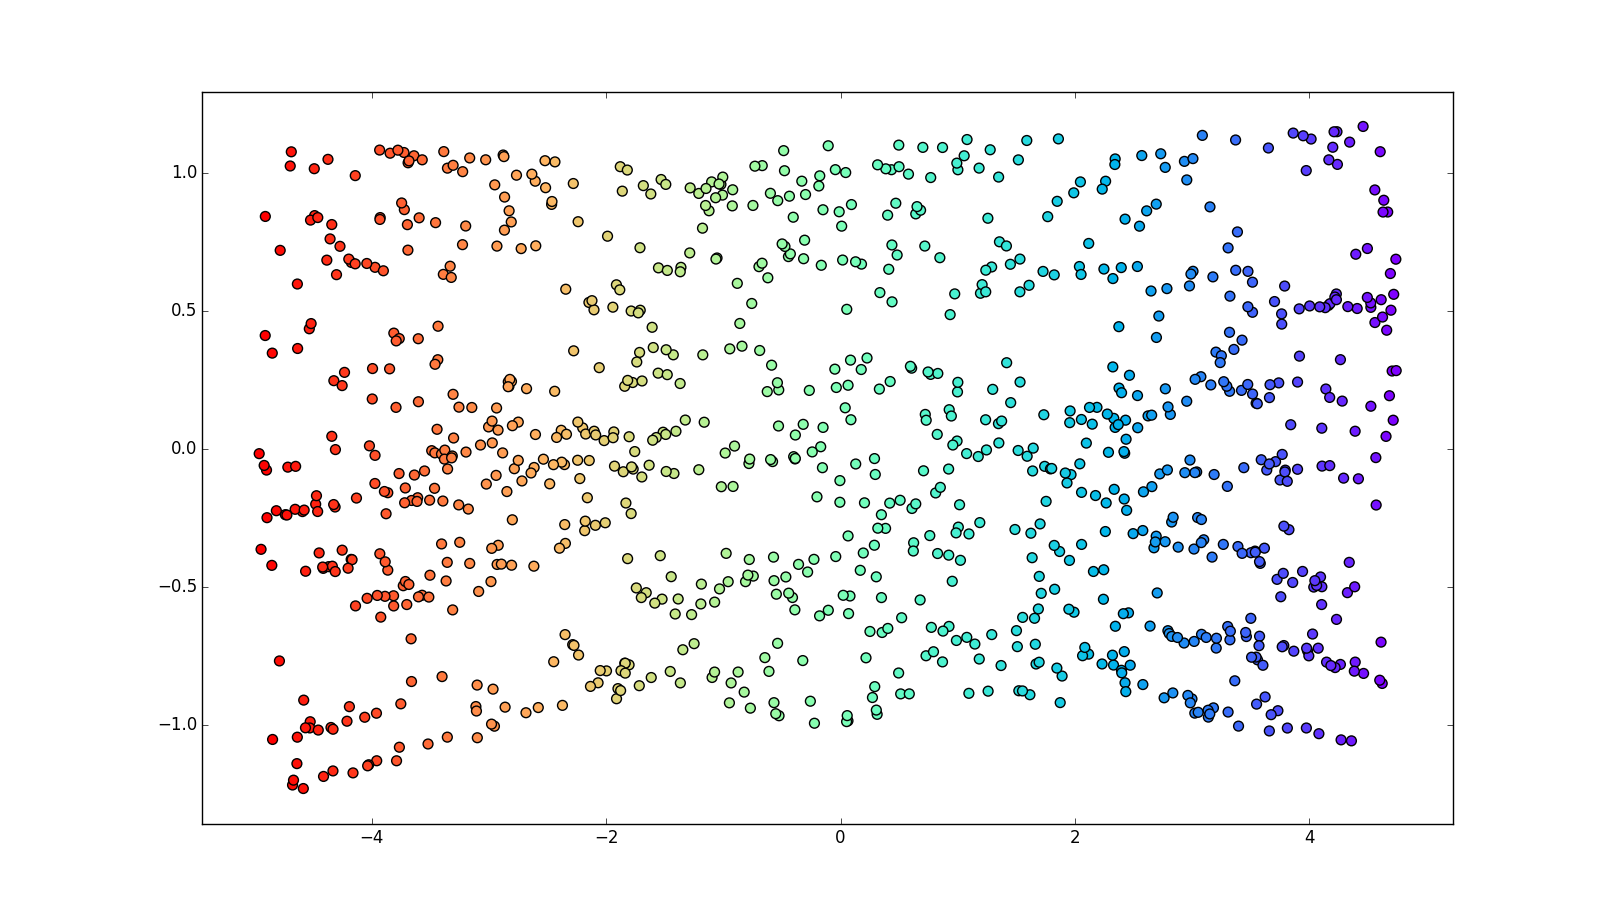
\includegraphics[width=\linewidth]{studying_isomap/embedding_2}
		\caption{$S$ reduced to two dimensions.}
		\label{fig:mani_s_reduced_1}
	\end{subfigure}%
	\begin{subfigure}{.5\linewidth}
		\centering
		\captionsetup{justification=centering}
		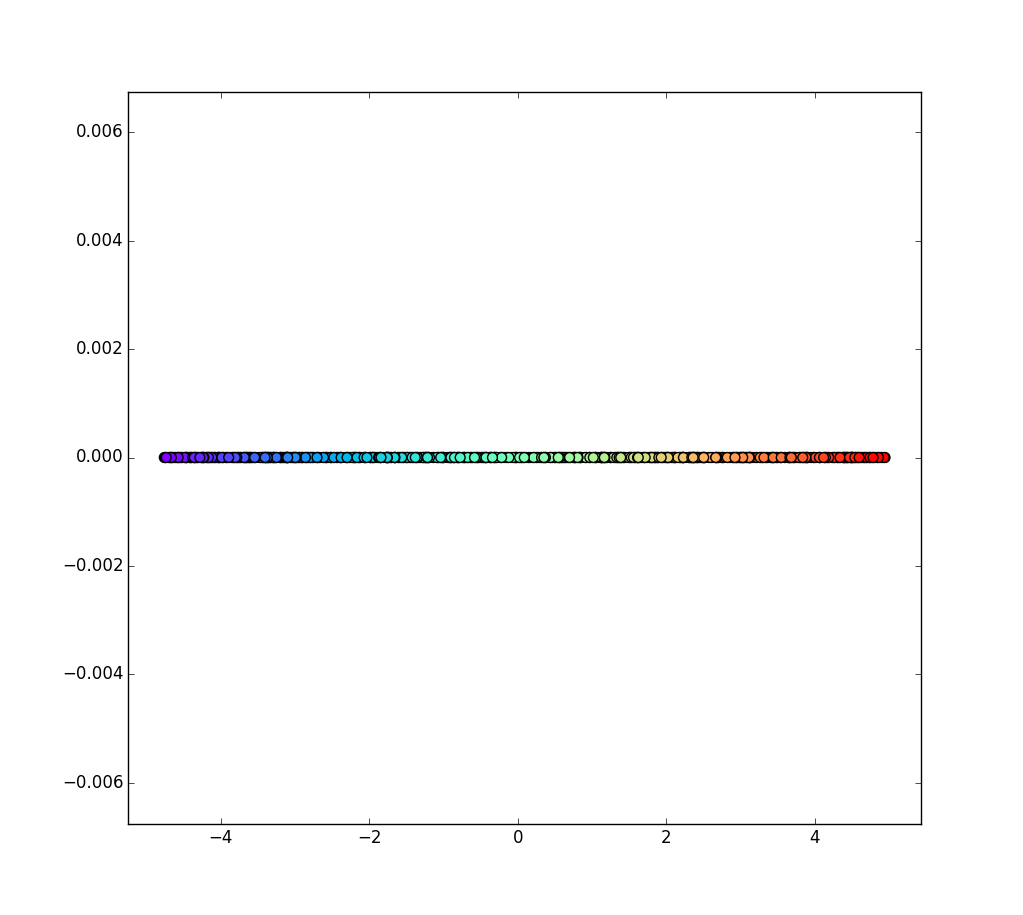
\includegraphics[width=.63\linewidth]{studying_isomap/embedding_1}
		\caption{$S$ reduced to one dimension.}
		\label{fig:mani_s_reduced_2}
	\end{subfigure}
\end{figure}

\newpage
\subsection{Formalization of the ISOMAP Algorithm}

Let $X$ be the original data set and $p \in \mathbb{R}$ the number of dimensions desired for the reduced data set, \cite{ten2000}

\begin{enumerate}
	\item Construct the weighted graph $G$ from the distances pairwise $\delta_{xy}, \forall (x, y) \in S \times S, x \ne y$ and find the graph $H$ by applying the \textbf{nearest-neighbor algorithm} on the graph $G$.

	\item Compute the shortest path graph $M$ between all pairs of nodes from graph $H$. This might be done by the \textbf{all-pairs Dijkstra's} or by the \textbf{Floyd-Warshall} algorithm.

	\item Use $M$ to construct the $p$-dimensional embedding using the \textbf{MDS} algorithm.
\end{enumerate}

\subsection{Computational Complexity}
\label{sec:isocomplexity}

If $n$ is the number of training samples, $f \in \mathbb{R}$ the number of features and $k \in \mathbb{R}$ the number of nearest neighbors:

\begin{enumerate}
	\item The time complexity associated with building the neighborhood graph is $O(n^2)$, whereas the space necessary to represent the distances kept is $n^2$.
	\item Algorithms for finding shortest path graph can be executed in-place and do not increase space complexity. Regarding time complexity, however:
	\begin{enumerate}
		\item Dijkstra's algorithm implementation using Fibonacci Heaps have time complexity $O(nk + n \log n)$. As the algorithm must be calculated for each node, this step has time complexity $O[n^2(k + \log n)]$.
		\item Alternatively, using the Floyd-Warshall algorithm, this step has time complexity equals to $O(n^3)$.
	\end{enumerate}
	\item Taking $O(n^3)$ time steps to calculate the spectral decomposition, MDS clearly is the bottleneck of the entire algorithm. \cite{cay2005} \cite{silva2002global} As for space complexity, $O(f^2 + nf)$ is required for storing the matrices $\Sigma$ and $U$.
\end{enumerate}

The time complexity of the ISOMAP algorithm (when using Dijkstra's) is, therefore, $O[n^2 + n^2(k + \log n) + n^3]$, and the space complexity is $O(n^2 + f^2 + nf)$.

\begin{experiment}[Timing the ISOMAP Algorithm]
	Consider the data set \textbf{Digits} with 1797 samples and 64 features. The following table indicates the time duration for each step of the ISOMAP algorithm when reducing Digits to 3 dimensions:

	\begin{table}[H]
		\centering
		\begin{tabular}{|l|r|}
			\hline
			\textbf{Pairwise distances from data set} & .44 s \\\hline
			\textbf{K Nearest Neighbors Search} & 1.3 s \\\hline
			\textbf{All Pairs Dijkstra's} & 51.44 s\\\hline
			\textbf{MDS} & 118.84 s \\\hline
			\textbf{Total Time} & 172.69 s \\\hline
		\end{tabular}

		\caption{Listing of time spent on each step of the ISOMAP algorithm.}
	\end{table}

	As expected, most of the time (68.81\%) was spent executing MDS.
\end{experiment}

In practice, ISOMAP's time complexity of $O[n^2 + n^2(k + \log n) + n^3]$ makes it unsuitable for data sets with high number of samples. This is illustrated in Shi and Gu's experiments: ISOMAP could not reduce data sets with more than 6000 samples in reasonable time. \cite{shi2012fast}

\begin{experiment}
	Let \textbf{Spam} be a data set with 4601 samples and 57 features. The table bellow describes the time necessary for the implemented ISOMAP and sk-ISOMAP (the algorithm from the \href{http://scikit-learn.org}{scikit-learn} library) to reduce Spam to 3 dimensions:

	\begin{table}[H]
		\centering
		\begin{tabular}{|c|c|}
			\hline
			\textbf{Algorithm} & Time \\\hline
			\textbf{ISOMAP} & 29.9 m \\\hline
			\textbf{sk-ISOMAP} & 10.76 s \\\hline
		\end{tabular}

		\caption{Timing the implemented ISOMAP and scikit-learn's implementation.}
	\end{table}

	The implemented ISOMAP required almost 30 minutes to reduce Spam.
	Surprisingly, scikit-learn's implementation executed incredibly fast. A set of factors contribute for this result:

	\begin{itemize}
		\item \textbf{Ball Tree} is used for efficient neighbor search (requiring only $O(f n \log k \log n)$ time steps).
		\item Many components in scikit-learn have python signatures, but are actually implemented in C, considerably increasing performance.
		\item ISOMAP is implemented as a kernel for the \textbf{KernelPCA} method. Further investigation is done in section \ref{sec:ISOMAP_extensions}.
	\end{itemize}

\end{experiment}

\subsection{Extensions}
\label{sec:ISOMAP_extensions}

\subsubsection{ISOMAP as a variation of Kernel PCA}

% TODO This description needs extensive refactoring.
While ``classic" PCA aims to find the principal components of the covariance matrix $\Sigma = \frac{1}{n} X^T X = \frac{1}{n} \sum_k x_{ik} \cdot x_{kj}, \forall (i, j) \in [0, |S|]^2$ of a centered data set $X$, it can be easily modified to attempt to do the same, but over the matrix $\Sigma' = \frac{1}{n} \sum_i \phi(x)_i \cdot \phi(y)_i = \frac{1}{n} \sum_i K(x, y)$, where $\phi \colon \mathbb{R}^f \to \mathbb{R}^p$ is a function that projects vectors in the original $f$-space to a different $p$-space and $K \colon \mathbb{R}^f \times \mathbb{R}^f \to \mathbb{R}$ is a kernel function. Such modification is named Kernel PCA.

In his paper, Ghodsi describes how MDS (and therefore, ISOMAP) is equivalent to Kernel PCA, given it is using the following kernel function: \cite{gho2006}

\begin{align*}
K_{ISOMAP} = -\frac{1}{2}H \delta^2 H
\end{align*}

Where $H \delta H$ is the double centered dissimilarity matrix, i.e, the double centered geodesic distances between samples found from the shortest-path graph.

An advantage of substituting the MDS algorithm by Kernel PCA is that the latter provides an embedding, i.e., a transformation matrix from the original space to the reduced one; whereas MDS only embeds the data set. \cite{ham2004kernel} However, Silva and Tenenbaum have shown that MDS's result can be used to reduce new samples (Landmark-MDS). \cite{silva2002global} More will be discussed in \ref{sec:lisomap}.

The figure bellow displays the reduction of the Swiss-roll data set done by the original implementation of ISOMAP (using MDS) and scikit-learn's implementation (using Kernel PCA). Clearly, they are identical.

\begin{figure}[H]
	\centering
	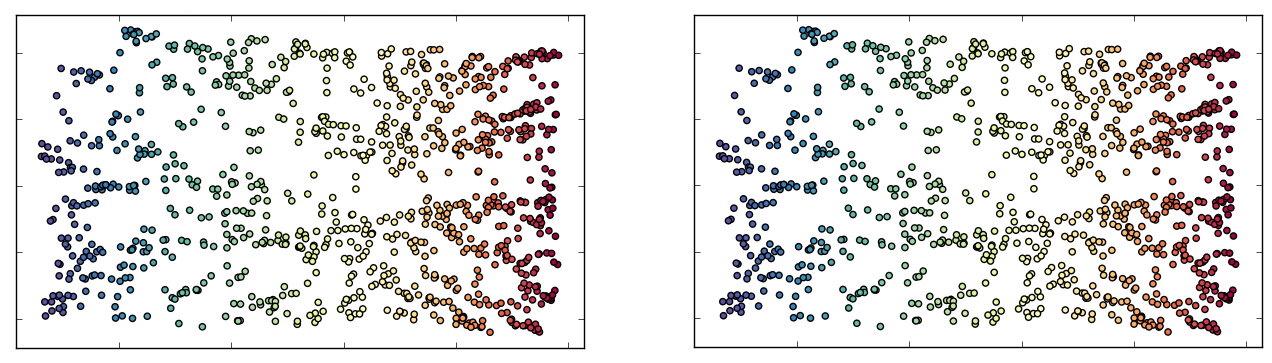
\includegraphics[width=\linewidth]{experiments/iso_comp_my_and_sklearn}
	\captionsetup{justification=centering}
	\caption{The embedded swiss-roll data set by the original and scikit-learn's implementation.}
\end{figure}

\subsubsection{Incremental ISOMAP}

The original ISOMAP algorithm reduces the data set in a single execution. Even its implementation with Kernel PCA will not update the reduction model if new data points are given, only reduce these points using the eigenvectors previously found. Therefore, updating ISOMAP reduction model requires recalculating it at every new data ``batch", which is very costly.

In order to allow ISOMAP to continuously learn from a stream of data, Incremental ISOMAP was proposed. \cite{law2006incremental} Relying on the fact that new data points will unlikely afect a large subsets of vertices, it selectively updates the structures kept by ISOMAP. The update is performed as it follows.

Let $[X]_{n \times f}$ be a data set with $n$ samples and $f$ features, $\delta_{ab}$ be the dissimilarity measure between two samples $a$ and $b$, $x_i$ be a sample in the nearest neighbor graph, $x_j$ a neighbor of $x_i$ such that their dissimilarity is higher among all $x_i$'s neighbors. Additionally, let $[Y]_{n \times d}$ be the embedding of $X$ in the $d$-dimensional space. Finally, consider $x_{n+1}$ a new sample to increment in the reduction model.

\begin{enumerate}
	\item The new sample $x_{n+1}$ will replace $x_j$ as a neighbor of $x_i$ if $\delta_{x_ix_{n+1}} < \delta_{x_ix_j}$. A list of added or removed edges should be stored.
	
	\item The update of the shorest-path graph:
	\begin{enumerate}
		\item For every edge $(x_i, x_j)$ removed, the shortest-path between any two points $(x_a, x_b)$ that contains $(x_i, x_j)$ must be updated. That involves applying a slightly modified Dijsktra's algorithm, which will focus on finding the paths from a given source $u$ and its unreached destination vertices, i.e., vertices $C(u)=\{c_i\}$ whose  shortest-paths $(u, c_i)$ contained a removed edge.
		
		\item The geodesic distances between all vertices and $x_{n+1}$ must then be calculated. Let $A$ be the set of added edges:
		\begin{align*}
			g[n+1, i] = g[i, n+1] = \min_{j \mid (n+1, j) \in A} (g[i, j]+w(j, n+1)),\forall i.
		\end{align*}
		
		All the added edges are incident on vertex $x_{n+1}$, naturally.  Calculating the shorest-path consists on considering two whichever edges $(a, x_{n+1}), (x_{n+1}, b)$ and relaxing the edge $(a, b)$ by considering the path $a \to x_{n+1} \to b$.
	\end{enumerate}
	
	\item Finally, the eigenvectors/eigenvalues of the inner product matrix $B_{new}$ (which contains the recently added sample $x_{n+1}$) can be found through an iterative scheme, where ``a good initial guess for the subspace of dominant eigenvectors is the column space of $Y$" \cite{law2006incremental} (the embedding before the $x_{n+1}$ increment).
	A better eigen-space for $B_{new}$, and thus $Y_{new}$ can be found by Subspace iteration together with Rayleigh-Ritz acceleration: \cite{law2006incremental} 
	\begin{enumerate}
		\item Let $Z = B_{new}Y$. Perform QR-decomposition on $Z$: $Z = B_{new}Y = QR$.
		
		\item Take $V=Q$ (remember that Q is intrinsically an orthogonal matrix) and $Z^*=V^TB_{new}V$. Perform spectral-decomposition of $[Z^*]_{d \times d}$ to find $\Lambda = diag(\lambda_i)$ and $V = [v_i]_{d \times d}$. This is significantly faster than directly decomposing $B_{new}$, considering the dimensions of both matrices. 

		\item $Y_{new} = [Y, y_{n+1}]^T$, where $y_{n+1}$ is the $d$-dimensional embedding of $x_{n+1}$:
		\begin{align*}
			y_{n+1} &= (\frac{1}{\sqrt{\lambda_1}} v_1 \cdot f, \dots, \frac{1}{\sqrt{\lambda_d}} v_d \cdot f) \\
			2f_i &\approx \frac{1}{n}[\sum_j g_{ij}^2 - \sum_{lj} g_{lj}^2 + \sum_l g_{l, n+1}^2] -g_{i, n+1}^2
		\end{align*}
	\end{enumerate}
\end{enumerate}

In regard to time complexity, considering $q$ the maximum degree of the vertices in the graph, $F$ is the set of pairs whose shortest path contained a removed edge and $H$ is the set of vertex pairs whose geodesic distances were modified, Incremental ISOMAP will require $O[q(|F|+|H|)]$ time steps in phase 1; $O[n^2(\log n + q)]$ in 2; and $O(n^2)$ in 3. The time complexity of the algorithm is, therefore, $O[q(|F|+|H|) + n^2(\log n + q + 1)]$.

\subsubsection{L-ISOMAP}
\label{sec:lisomap}

ISOMAP's time complexity dependents mainly on the number of samples. Remember: for $N$ samples, ISOMAP will require $O[n^2(\log n + k)]$ and $O[n^3]$ time operations to compute the shortest-paths and eigenvectors/values, respectively.

Landmark ISOMAP aims to reduce the complexity of the algorithm by finding the dissimilarities between $n$ landmarks (a small subset of samples) and all the original samples. Its complexity can then be reduced to $O[n^2(\log N + k) + n^2N]$. If $n \ll N$, this represents a expressive performance improvement. \cite{silva2002global}

Let $X$ be the initial data set of interest, $l$ be the dimensionality to which $X$ should be reduced and $\epsilon > 0 \in \mathbb{N}$ a number to ``ensure stability". \cite{silva2002global} L-ISOMAP is defined as it follows.

\begin{enumerate}
	\item Select $n$ random samples from $X$, such that $n > l + 1 + \epsilon$.
	\item Calculate the nearest-neighbors of each selected samples (all the original samples should be considered as neighbors).
	\item Calculate the shortest-paths from the neighborhood graph obtained in the previous step and the dissimilarity matrix $[\delta]_{n \times N}$.
	\item Perform Landmark MDS, an slightly modifed MDS:
	\begin{enumerate}
		\item Apply classical MDS to the submatrix of landmarks $[\delta]_{n \times n}$.
		\item Embbed the remaining points through:
		\begin{align*}
			y &= -\frac{1}{2} L^{-1}  (\Delta_x - \bar{\Delta}_n)\\		
			y &= -\frac{1}{2} \colvec{4}{\frac{v_1^T}{\sqrt{\lambda_1}}}{\frac{v_2^T}{\sqrt{\lambda_2}}}{\dots}{\frac{v_n^T}{\sqrt{\lambda_n}}} (\Delta_x - \bar{\Delta}_n)\\
		\end{align*}
		Where $\Delta_x$ is the square dissimilarity column vector from sample $x$ to all landmarks and $\bar{\Delta}_n$ the vector containing the column mean of $\Delta_n$ (the square dissimilarity matrix between landmarks).
	\end{enumerate}
\end{enumerate}

\subsubsection{p-ISOMAP}

The embedding found by ISOMAP is strongly depentend of the parameters $k$ or $\epsilon$. When these parameters are too small, the neighborhood graph extracted might be disconnected, causing the dissimilarity between some some vertices to be infinite. On the other hand, when the parameters are too big, vertices from different neighborhoods are prone to stay connected, preventing the manifold to be ``unfolded". Hence the importance of choosing appropriate parameters. However, in many cases, these ``appropriate" paramaters might not be not evident. Hence the interest of developing a parameterless ISOMAP.

p-ISOMAP is an extension that automatically selects the parameters $k$ or $\epsilon$. \cite{choo2010p} Assuming an result of ISOMAP for a particular parameter value is available, a new parameter will be considered and p-ISOMAP will iteratively update the soluton by:
\begin{enumerate}
	\item Adding/removing neighbors for every vertex in the neighborhood graph regarding the new parameter. This operation has time complexity $O(n \max_i |\Delta e_i|)$, where $|\Delta e_i|$ is the number of inserted/removed edges associated with sample $x_i$.
	
	\item Update the shortest-paths described by the pairs of vertices in $F \subset Q$, where $Q$ is the set of all pairs of vertices and $F$ is the set of pairs associated with the updated edges in the previous step.
	\begin{enumerate}
		\item	If the parameter value increased in comparison to the previous one, edges might have been added. Updating the shortest-path tree consists in simply relaxing edges associated with any of the vertices in the pairs of $F$. The time complexity is loosely bounded by $O(|A|q|F|)$, where $|A|$ is the number of inserted edges and $q$ is the maximum degree of vertices in G.
		
		\item If the parameter was decreased, then edges might have been removed and all pairs of vertices whose shortest-paths contain those edges are added to $F$. Identifying $F$ can be done in $O(n^2)$ times steps to execute, given some optimzation (see \cite{choo2010p}). Now, Dijkstra's can be selectively performed, requiring $O(n \max_i (|E_i'| \log |V_d(i)| + |E_i''|)$, where, given a vertex $x_i$, $V_d(i)=\{x_j | (x_i, x_j) \in F\}$, $E_i'$ is the set of edges connecting whichever pair of vertices in $V_d(i)$ and $E_i''$ is the set of edges connecting the vertices $x_a$ and $x_b$ such that $x_a$ is in $V_d(i)$ and $x_b$ is not.
	\end{enumerate}

	\item Finally, the last step is to update the eigenvectors and eigenvalues associated with the matrix $B$. They can be approximated using the Lanczos algorithm, an iterative refining method that takes an initial solution candiadate. Officially, the time complexity of Lanczoz algorithm is $O(n^2)$. \cite{chen2004machine} Yet, its timeframe for convergence also strongly depends on the solution candidate given. Assuming the previous inner matrix and the current one are similar, one might use the previous eigenvalues/vectors found as candidate. In this scenario, Lanczoz's will likely finish much faster than other algorithms.
\end{enumerate}

The experiments presented in \cite{choo2010p} have shown p-ISOMAP consistently maintaining a better performance than regular ISOMAP for data sets with a samples count varying between 500 and 3500.
Additionally, the experiments have also demonstrated how p-ISOMAP performance is sensible to high variances of $K$ and $\epsilon$ values.

\subsection{Evaluating Reductions}

ISOMAP's aim is to ``unfold" the data set and, of course, it might distort dissimilarities between samples in the process. Hence drastically increasing Kruskal's stress. Clearly, this measure is unsuitable for evaluating ISOMAP. As proposed by L. Shi and J. Gu, Kruskal's stress can be easily updated to match ISOMAP nature. That is, to preserve dissimilarities within neighborhoods: \cite{shi2012fast}

Let $X_{n \times f}$ be a data set with $n$ samples and $f$ dimensions, $Y_{n \times p}$ its reduction to $p$ dimensions, and $\delta_{ij}$ and $\hat{\delta}_{ij}$ the dissimilarity measurements defined for all samples $i$ and $j$ in both $X$ and $Y$. Furthermore, given a sample $i$ and $\beta \in \mathbb{N} \mid \beta \le n$, take $\Omega=K \bigcup \Theta$, where $K$ is the set containing the nearest neighbors of $i$ and $\Theta$ is a set of random samples such that $|\Theta| \le \beta \le n$:
\begin{align*}
	Stress_{ISOMAP} &= [\frac{\sum_i \sum_{j \in \Omega} (\delta_{ij} - \hat{\delta}_{ij})^2}{\sum_i \sum_{j \in \Omega} \delta_{ij}^2}]^{\frac{1}{2}}
\end{align*}

\subsection{Applicability and Limitations}

It is quite clear that ISOMAP outperforms PCA on the data set $S$. Unfortunately, this cannot be projected for a generic case considering the strict and artificial nature of $S$. In real-world data sets, the application of ISOMAP may lead to poor low-dimensional embeddings. \cite{herik2009} Bellow are listed some the issues that have great influence over ISOMAP's results:
\begin{description}
	\item[Manifold Assumption] It refers to the initial assumption that the data lies on a low-dimensional manifold. Although wildly exploited by many authors, it is difficult to assert whether such assumption holds or not in real-world data sets. \cite{lin2008riemannian} Furthermore, even if the data roughly lies on a manifold, discontinuities in the data pattern can characterize the manifold as non-smooth. In these situations, graphs with edges that disrespect locality would be extracted and, hence, poor low-dimensional representations are likely to be produced.

	\newpage

	\item[Manifold Convexity] "ISOMAP relies on the data being geodesically convex." \cite{donoho2002does} This issue becomes clear when dealing with data sets with ``holes" in it that occupy sufficiently large areas, resulting in a neighborhood graph with great disconnected areas that require paths with great curvature to get around. Lerman demonstrated how reducing non-convex data sets with ISOMAP can easily yield distorted results: \cite{lerman2005}
	\begin{figure}[H]
		\centering
		\begin{subfigure}[H]{.45\linewidth}
			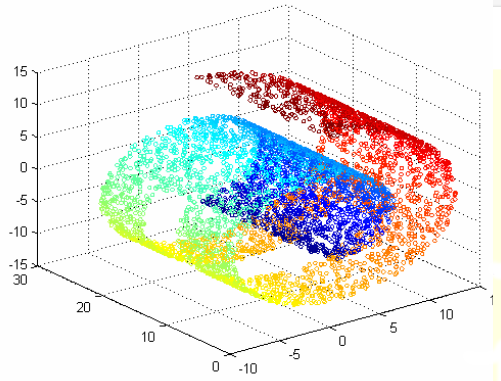
\includegraphics[width=\linewidth]{img/convexity/original.png}
			\captionsetup{justification=centering}
			\caption{The non-convex Swiss-roll.}
		\end{subfigure}
		~
		\begin{subfigure}[H]{.45\linewidth}
			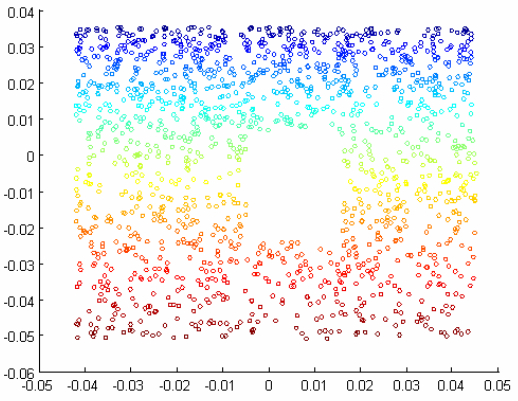
\includegraphics[width=\linewidth]{img/convexity/expected.png}
			\captionsetup{justification=centering}
			\caption{The expected reduction.}
		\end{subfigure}
		\newline\newline

		\begin{subfigure}[H]{.45\linewidth}
			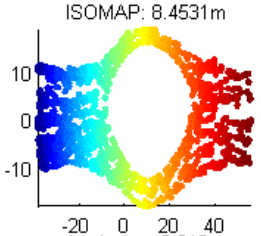
\includegraphics[width=\linewidth]{img/convexity/actual.png}
			\captionsetup{justification=centering}
			\caption{The actual reduction.}
		\end{subfigure}
	\end{figure}

	\newpage
	\item[Noise] Noise in data is expressed by samples that somehow diverge from their neighborhood (outliers). As these samples become farthest from its original neighborhood, the chances of being linked to samples from other neighborhood increase, possibly decreasing the quality of the solution. A possible solution is to remove these samples during the pre-processing stage \cite{herik2009}.

	The image bellow illustrates an attempt to use ISOMAP to reduce the $M_{n=.4}$, which is the Swiss-roll data set subjected to a noise factor of $.8$:

	\begin{figure}[H]
		\centering
		\begin{subfigure}{.45\linewidth}
			\centering
			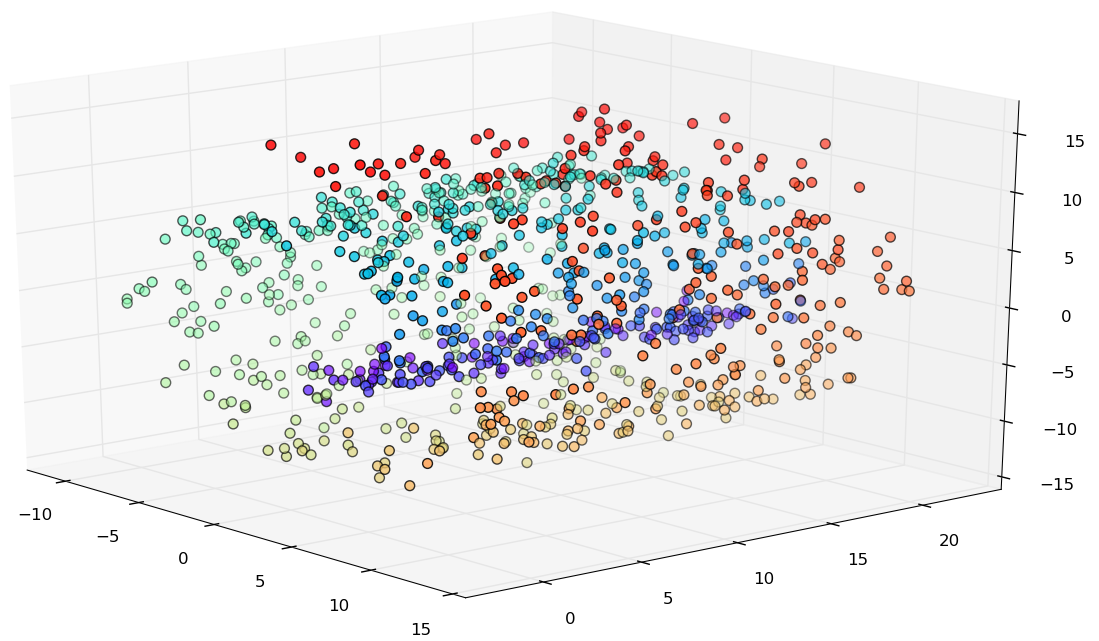
\includegraphics[width=\linewidth]{img/noise/sr/1}
			\captionsetup{justification=centering}
			\caption{The data set $M_{n=.8}$.}
		\end{subfigure}~
		\begin{subfigure}{.40\linewidth}
			\centering
			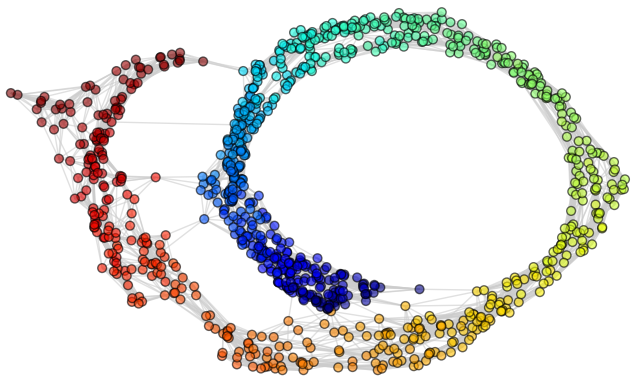
\includegraphics[width=\linewidth]{img/noise/sr/3}
			\captionsetup{justification=centering}
			\caption{The neighborhood graph extracted from $M_{n=.8}$.}
			\label{fig:noise_3}
		\end{subfigure}
		\newline\newline\newline
		\begin{subfigure}{.45\linewidth}
			\centering
			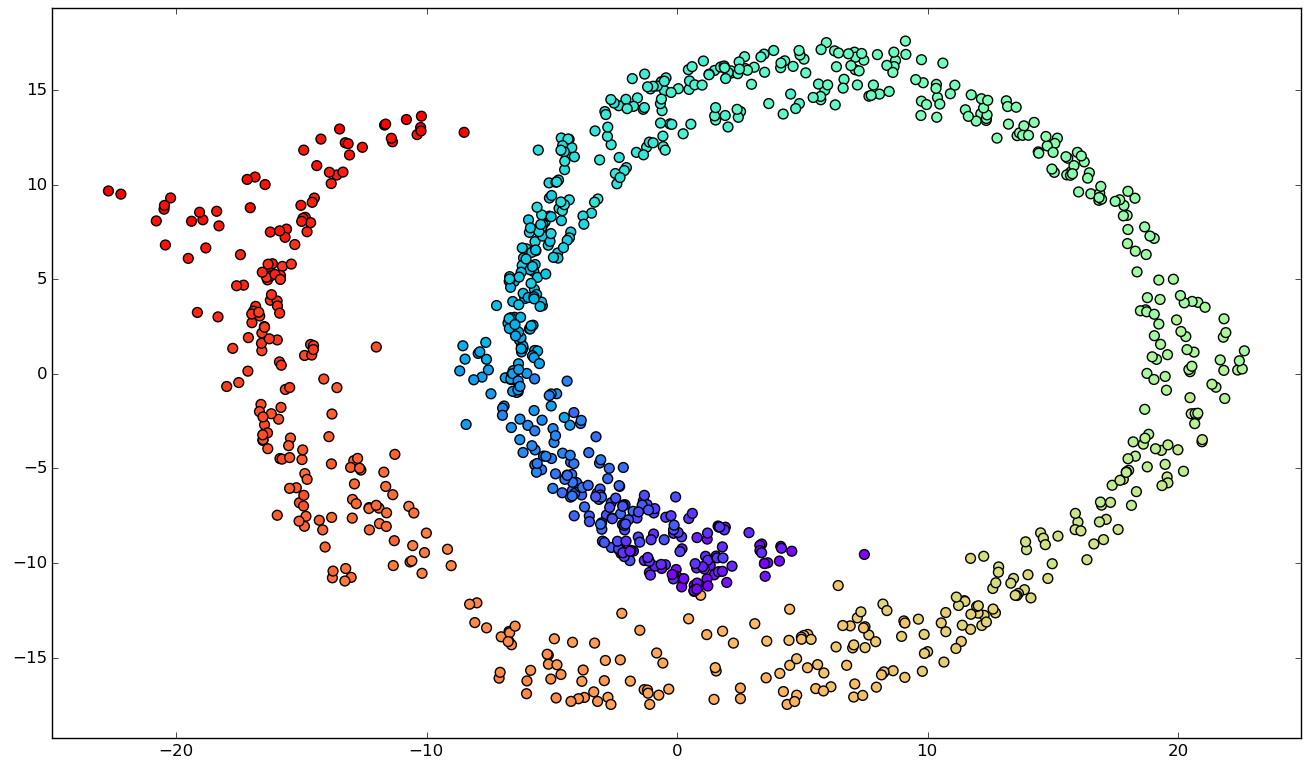
\includegraphics[width=\linewidth]{img/noise/sr/2}
			\captionsetup{justification=centering}
			\caption{$M_{n=.8}$ reduced.}
			\label{fig:noise_2}
		\end{subfigure}
		\captionsetup{justification=centering}
		\caption{The ISOMAP applied on a noisy data set.}
	\end{figure}

	Observe how some outliers were sufficiently far from their original neighborhood in the graph \ref{fig:noise_3}, to the point that Nearest-Neighbor Search maintained the edge between them and samples of completely different colors. MDS then attempted to maintain this dissimilarity, resulting in a deformed reduction (figure \ref{fig:noise_2}).
\end{description}

\newpage
\section{Classification and Regression Over Data Sets Reduced with ISOMAP}

Just as in \ref{sec:experiments_linear_ds}, this section reports reduction, classification and regression experiments made in common data sets, following the same format as before.

\subsection{The Swiss Roll Data Set}

\begin{figure}[H]
	\centering
	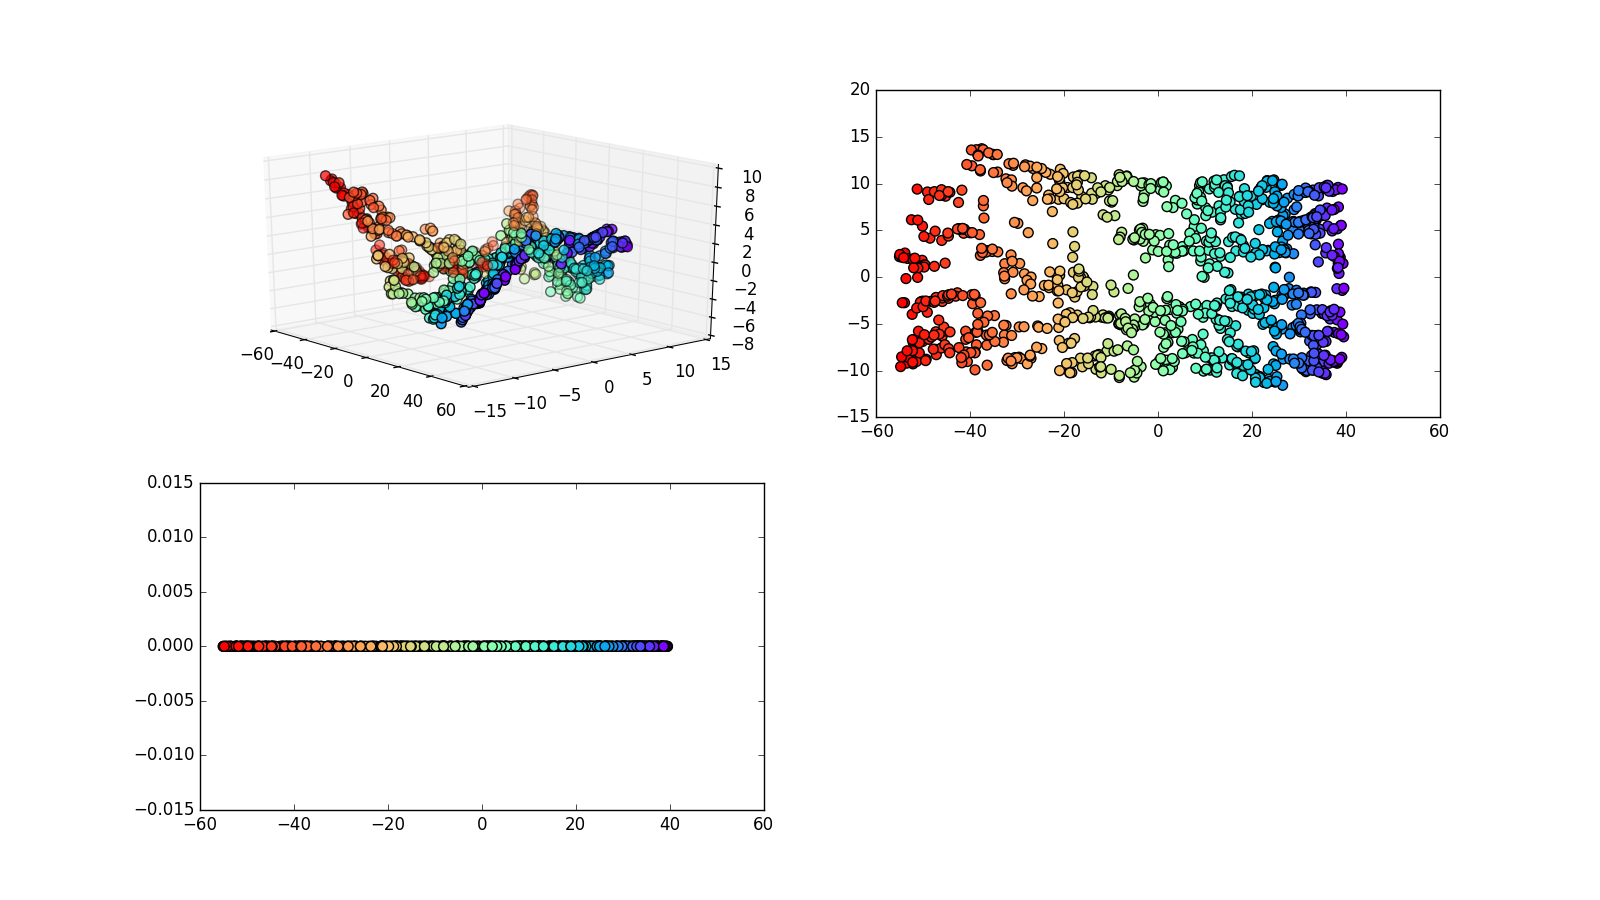
\includegraphics[width=.95\linewidth]{experiments/iso_swiss}
	\captionsetup{justification=centering}
	\caption{The Swiss Roll data set and its reductions to 2 and 1 dimensions, respectively.}
\end{figure}

\begin{table}[H]
	\centering
	\begin{tabular}{|c|c|c|c|}
		\hline
		& \textbf{Orig. $\mathbb{R}^3$} & \textbf{$\mathbb{R}^2$} & \textbf{$\mathbb{R}$} \\\hline
		\textbf{Prediction accuracy}   & 1            & 1             & 1     \\\hline
		\textbf{GridSearch time} & 15.53 s   & 415.72 s  & 387.98 s  \\\hline
		\textbf{Reduction time}  & -         & 0.51 s       & 0.48 s     \\\hline
		\textbf{Data size}          & 23.44 KB & 15.62 KB  & 7.81 KB   \\\hline
	\end{tabular}

	\caption{Description of predictions and reduction performance for Swiss Roll.}
\end{table}

\subsection{The Iris Flower Data Set}

Once again, the Iris flower data set, containing 150 samples and 5 features.

\begin{figure}[H]
	\centering
	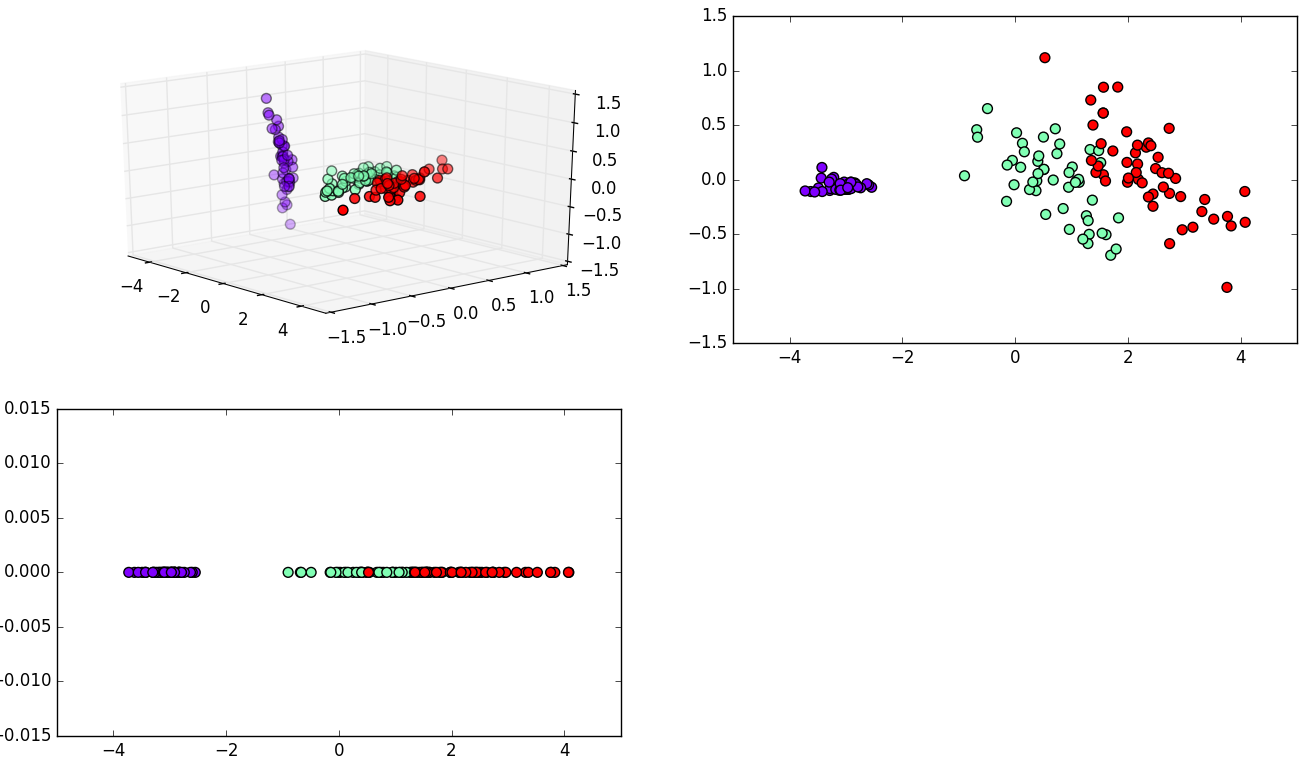
\includegraphics[width=\linewidth]{experiments/iso_iris}
	\captionsetup{justification=centering}
	\caption{The Iris data set and its reductions to 3, 2 an 1 dimensions, respectively.}
\end{figure}

\begin{table}[H]
	\centering
	\begin{tabular}{|c|c|c|c|c|}
		\hline
		& \textbf{Orig. $\mathbb{R}^4$} & \textbf{$\mathbb{R}^3$} & \textbf{$\mathbb{R}^2$} & \textbf{$\mathbb{R}$} \\\hline
		\textbf{Prediction accuracy}   & .99      & .97  s             & .97             & .89           \\\hline
		\textbf{GridSearch time}           & .27 s   & .25 s              & .25 s         & .27 s        \\\hline
		\textbf{Reduction time}             & -           & .19 s              & .19 s          & .36 s        \\\hline
		\textbf{Stress}                                  & -           & .474525      & .569293   & .655614 \\\hline
		\textbf{Data size}                           & 4.69 KB & 3.52 KB  & 2.34 KB   & 1.17 KB  \\\hline
	\end{tabular}

	\caption{Description of predictions and reduction performance for Iris.}
\end{table}

\newpage
\subsection{The Glass Data Set}

The Glass data set contains 214 samples and 11 features, were the first one is the identification number of a given sample and the last one is the class to which that sample belongs.

\begin{figure}[H]
	\centering
	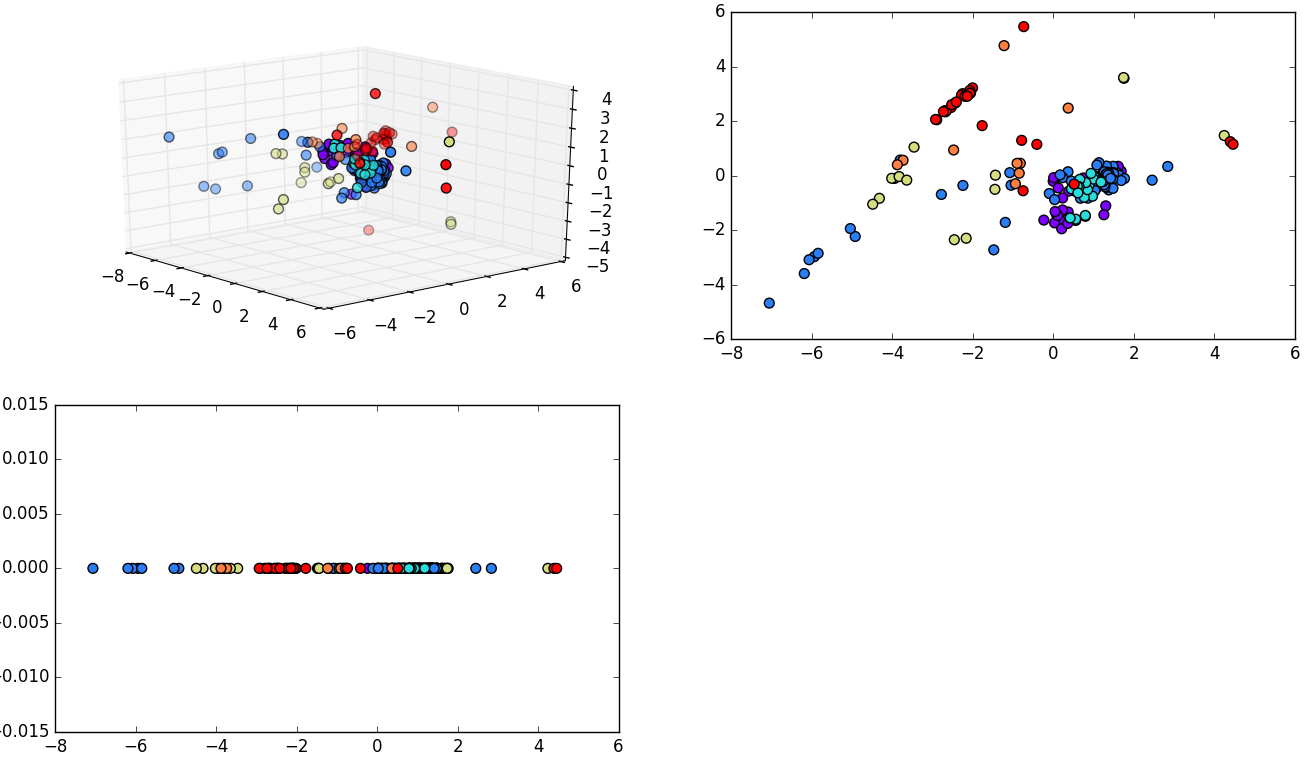
\includegraphics[width=\linewidth]{experiments/iso_glass}
	\captionsetup{justification=centering}
	\caption{The Glass data set and its reductions to 3, 2 an 1 dimensions, respectively.}
\end{figure}

\begin{table}[H]
	\centering
	\begin{tabular}{|c|c|c|c|c|c|}
		\hline
		& \textbf{Orig. $\mathbb{R}^{9}$} & \textbf{$\mathbb{R}^8$} & \textbf{$\mathbb{R}^6$} & \textbf{$\mathbb{R}^4$}  & \textbf{$\mathbb{R}^3$} \\\hline
		\textbf{Prediction accuracy}   & .64 & .63  & .66 & .65  & .65 \\\hline
		\textbf{GridSearch time} & .36 s & .35 s   & 2.77 s & 2.36 s & 1.26 s  \\\hline
		\textbf{Reduction time}  & -  & .66 s & .65 s & .68 s    & .64 s     \\\hline
		\textbf{Stress} & - & .513717 & .462840 & .362030 & .306092 \\\hline
		\textbf{Data size}          & 15.05 KB & 13.37 KB & 10.03 KB & 6.69 KB & 5.02 KB   \\\hline
	\end{tabular}

	\caption{Description of predictions and reduction performance for Glass.}
\end{table}

\newpage
\subsection{The Digits Data Set}

\begin{figure}[H]
	\centering
	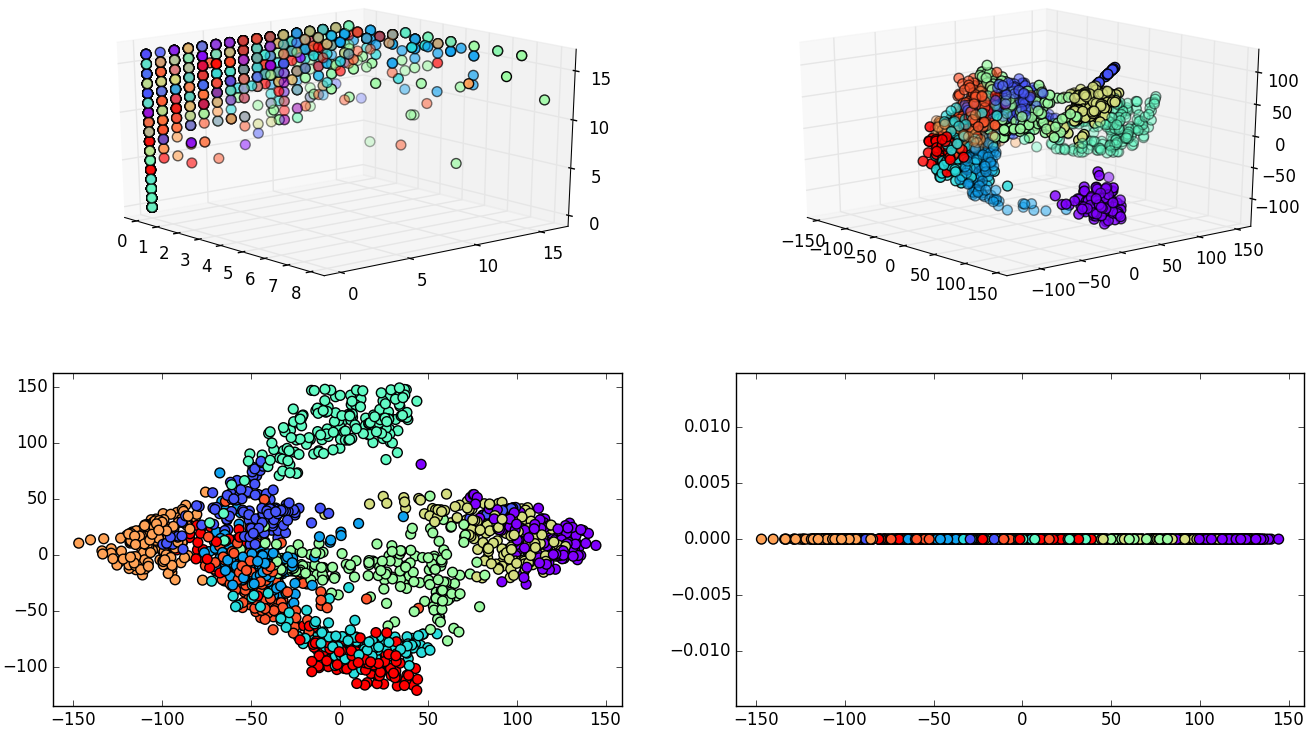
\includegraphics[width=\linewidth]{experiments/iso_digits}
	\captionsetup{justification=centering}
	\caption{Digits data set and its reductions to 3, 2 and 1 dimension, respectively.}
	\label{fig:dsdigitsiso}
\end{figure}

\begin{table}[H]
	\centering
	\begin{tabular}{|c|c|c|c|c|c|}
		\hline
		& \textbf{Orig. $\mathbb{R}^{64}$} & \textbf{$\mathbb{R}^{10}$} & \textbf{$\mathbb{R}^3$} & \textbf{$\mathbb{R}^2$} & \textbf{$\mathbb{R}$} \\\hline
		\textbf{Pred. accuracy}   & .98 & .96 & .91 & .69 & .45 \\\hline
		\textbf{GridSearch time} & 12.22 s & 98.08 s & 287.46 s & 630.47 s & 949.88 s \\\hline
		\textbf{Reduction time}  & - & 5.43 s & 2.72 s & 2.71 s & 2.04 s \\\hline
		\textbf{Data size} & 898.50 KB & 140.39 KB & 42.12 KB & 28.08 KB & 14.04 KB \\\hline
	\end{tabular}

	\caption{Description of predictions and reduction performance for Digits.}
\end{table}

Notice that the data set was reduced to only 3 dimensions, while maintaining 91\% of accuracy (remember that dimensionality reduction with PCA would reduce accuracy to 74\%). Accuracy loss is still observable when reducing it to two or one dimensions, although it is less intense than losses caused by linear reduction.

\newpage
\subsection{The Dermatology Data Set}

The Dermatology data set, composed by 366 samples and 35 features. Here, the target is to correctly diagnose the erythemato-squamous diseases.

\begin{figure}[H]
	\centering
	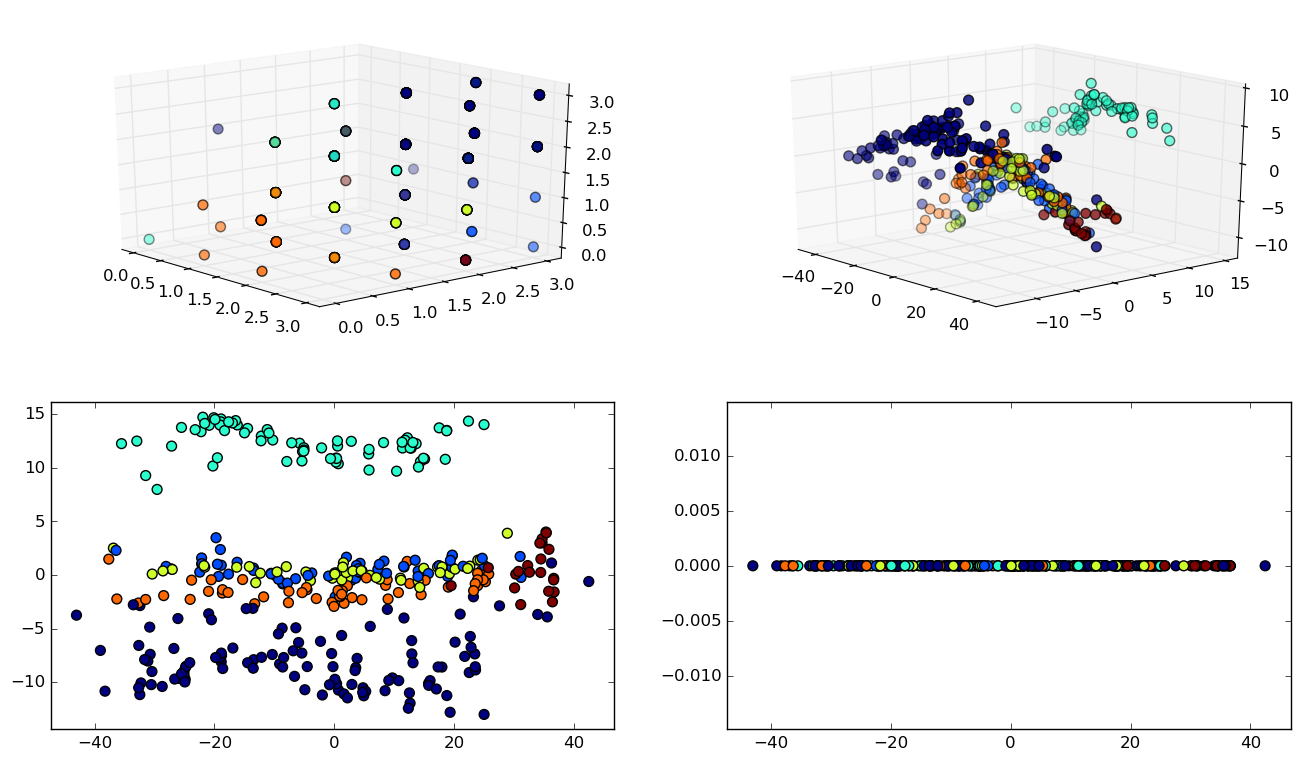
\includegraphics[width=\linewidth]{experiments/iso_dermatology}
	\captionsetup{justification=centering}
	\caption{The Dermatology data set and its reductions to 3, 2 an 1 dimensions, respectively.}
\end{figure}

\begin{table}[H]
	\centering
	\begin{tabular}{|c|c|c|c|c|c|}
		\hline
		& \textbf{Orig. $\mathbb{R}^{34}$} & \textbf{$\mathbb{R}^{20}$} & \textbf{$\mathbb{R}^{10}$} & \textbf{$\mathbb{R}^3$} & \textbf{$\mathbb{R}^2$} \\\hline
		\textbf{Prediction accuracy}  & .953552 & .915301 & .907104 & .827869 & .784153 \\\hline
		\textbf{GridSearch time} & .67 s & .76 s & 2.06 s & 27 s & 44.1 s  \\\hline
		\textbf{Reduction time}  & -         & 5.1 s & 4.89 s & 4.91 s & 4.96 s    \\\hline
		\textbf{Stress} & - & .771817 & .597724 & .465458 & .416376 \\\hline
		\textbf{Data size}          & 97.22 KB & 57.19 KB & 28.59 KB  & 8.59 KB & 5.72 KB  \\\hline
	\end{tabular}

	\caption{Description of predictions and reduction performance for Dermatology.}
\end{table}

\newpage
\subsection{The Leukemia Data Set}

Extracted from \href{http://mldata.com}{mldata}, the Leukemia data set contains 72 samples and 7130 features. The first 7129 features are expression levels of the genes in a given patient. The 7130th feature $t \in \{-1, 1\}$ indicate which of two variants of leukemia is present in the sample (AML, 25 samples, or ALL, 47 samples). \cite{on:duc_ds}

The Results in this experiment are quite impressive: although visualization has barely changed from 7129 to 3 dimensions, a 7129-dimensional space was reduced to a 10-dimensional one with only 10\% of accuracy loss.

\begin{figure}[H]
	\centering
	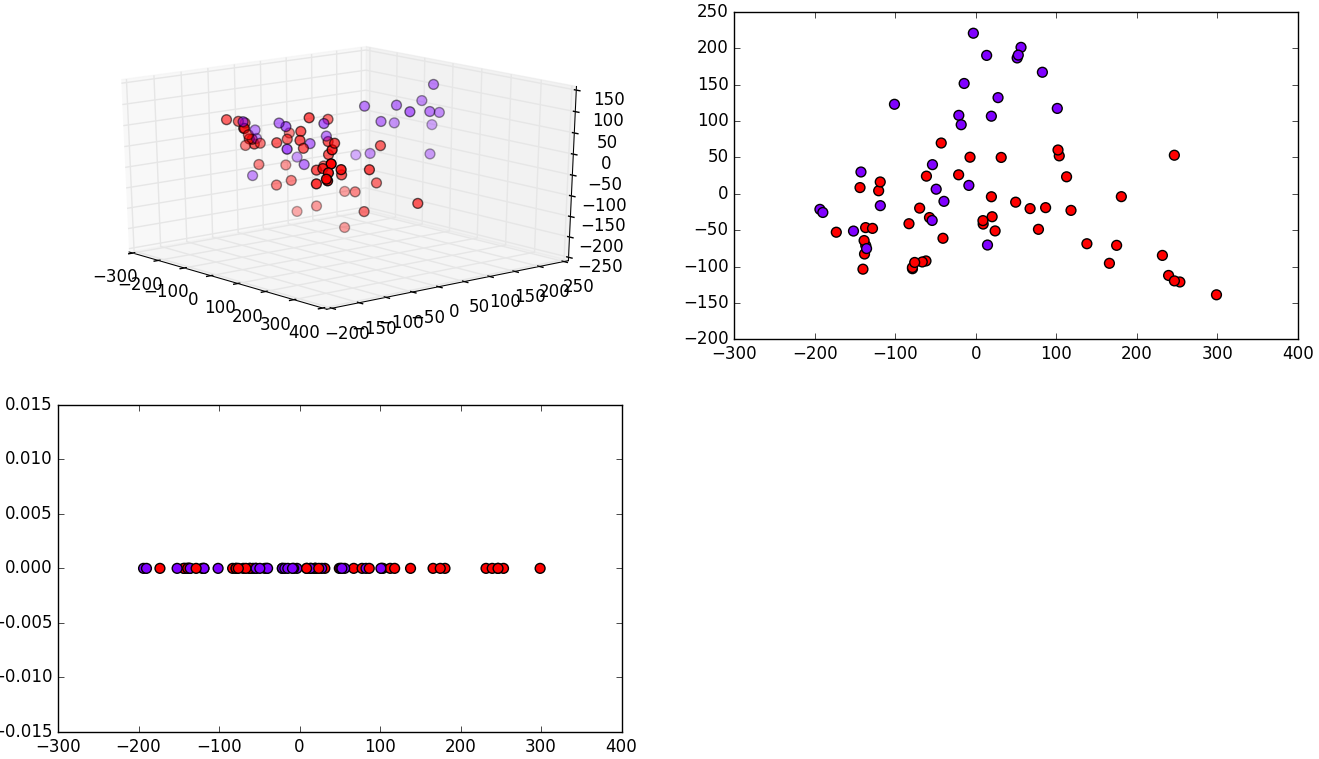
\includegraphics[width=.9\linewidth]{img/experiments/iso_leukemia}
	\captionsetup{justification=centering}
	\caption{The Leukemia data set and its reduction to 3, 2 and 1 dimensions, respectively.}
	\label{fig:leukemiads}
\end{figure}

\begin{table}[H]
	\centering
	\begin{tabular}{|c|c|c|c|c|}
		\hline
		& \textbf{Orig. $\mathbb{R}^{7129}$} & \textbf{$\mathbb{R}^{30}$} & \textbf{$\mathbb{R}^{20}$} & \textbf{$\mathbb{R}^{10}$} \\\hline
		\textbf{Pred. accuracy}    & .99 & .88 & .85 & .88 \\\hline
		\textbf{GridSearch time}   & 2.42 s & .26 s & .26 s & 141.13 s \\\hline
		\textbf{Reduction time}    & - & .06 s & .04 s & .04 s \\\hline
		\textbf{Data size}         & 4010.06 KB & 16.88 KB & 11.25 KB & 5.62 KB \\\hline
	\end{tabular}
	\captionsetup{justification=centering}
	\caption{Description of predictions and reduction performance for Leukemia data set.}
\end{table}

\subsection{The WDBC Data Set}

The Wisconsin Diagnostic Breast Cancer (WDBC) data set, containing 596 samples and 32 features computed from a breast mass. WDBC has benign 357 samples and 212 malignant. During this experiment, the first feature was disregarded, as it represents the identification numbers of the samples.

Regarding the experiment, observe how prediction accuracy consistently increased when the data set was reduced.

\begin{figure}[H]
	\centering
	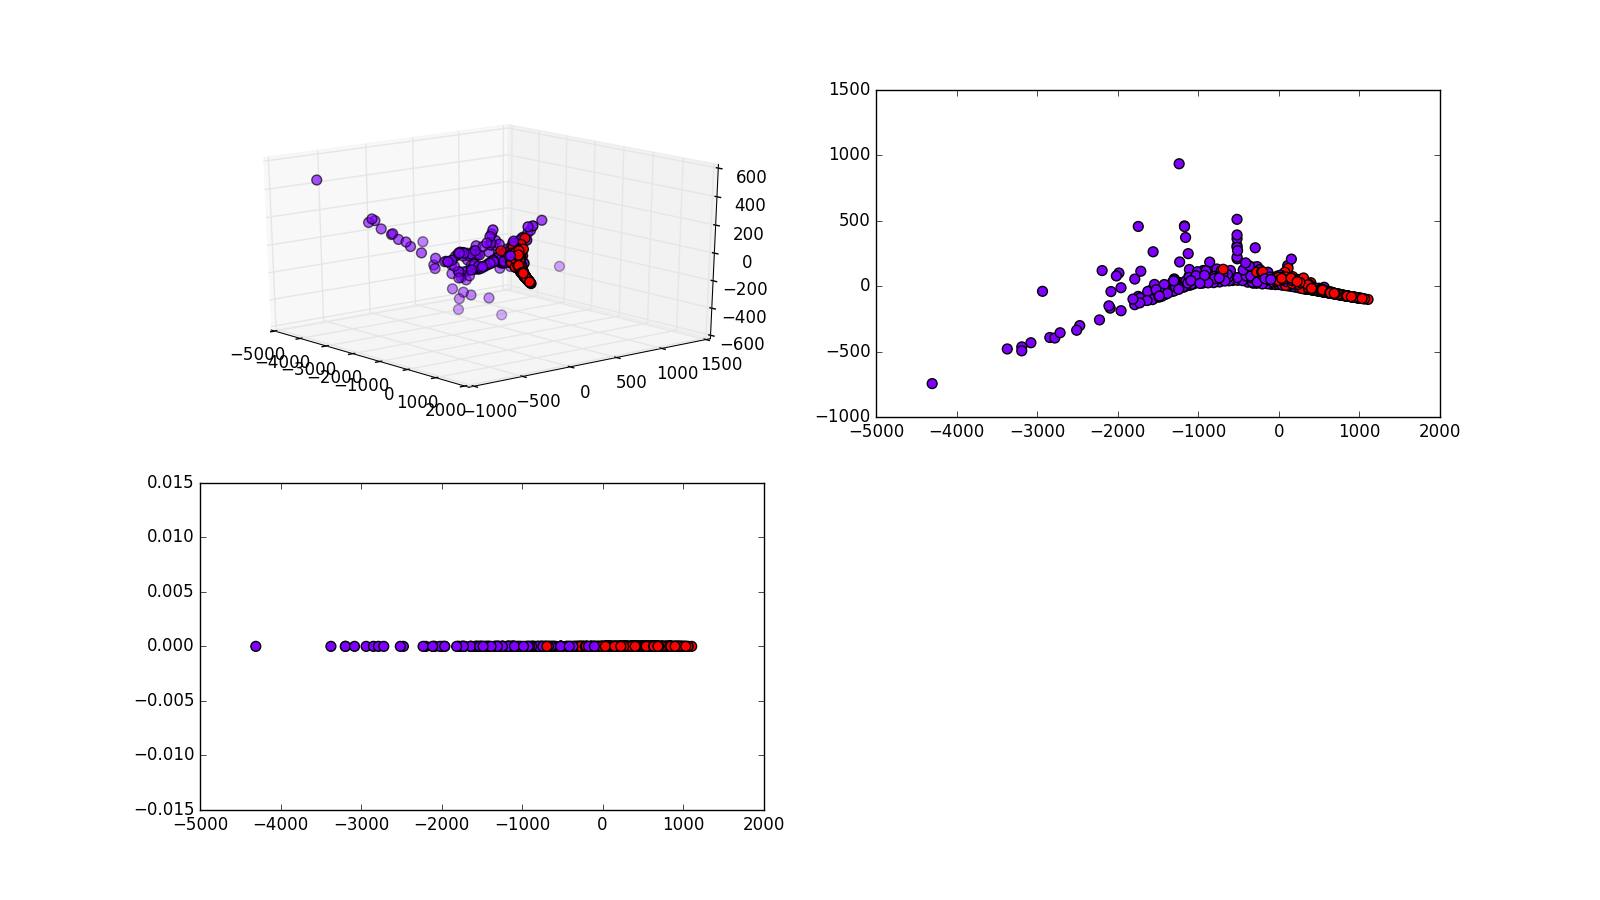
\includegraphics[width=.9\linewidth]{img/experiments/iso_wdbc}
	\captionsetup{justification=centering}
	\caption{The WDBC data set and its reduction to 3, 2 and 1 dimensions, respectively.}
	\label{fig:iso_wdbc}
\end{figure}

\begin{table}[H]
	\centering
	\begin{tabular}{|c|c|c|c|c|c|}
		\hline
		& \textbf{Orig. $\mathbb{R}^{30}$} & \textbf{$\mathbb{R}^{20}$} & \textbf{$\mathbb{R}^{10}$} & \textbf{$\mathbb{R}^{3}$} & \textbf{$\mathbb{R}^{2}$} \\\hline
		\textbf{Pred. accuracy}    & .63 & .89 & .8963 & .8998  & .8998 \\\hline
		\textbf{GridSearch time}   & 0.58 s & 0.46 s & 0.36 s & 0.36 s & 0.36 s \\\hline
		\textbf{Reduction time}    & - & 3.31 s & 3.25 s & 3.26 s & 3.31 s \\\hline
		\textbf{Stress} & - & .53 & .465460 & .378905 & .352277 \\\hline
		\textbf{Data size}  & 133.36 KB & 88.91 KB & 44.45 KB & 13.34 KB & 8.89 KB \\\hline
	\end{tabular}
	\captionsetup{justification=centering}
	\caption{Description of predictions and reduction performance for Leukemia data set.}
\end{table}

\newpage
\subsection{Diabetes Data Set}

With 9 features observed from 768 samples collected from residents of Arizona, USA, the Diabetes data set seeks to diagnose whether a patient (sample) shows signs of diabetes (class 1) according to World Health Organization criteria or not (class 0). Is is also important to mention that only 268 samples belong, in fact, to class 1.

In this experiment, Diabetes was compressed to one forth of its original size (48 KB to 12 KB), and no significant prediction accuracy was lost.

\begin{figure}[H]
	\centering
	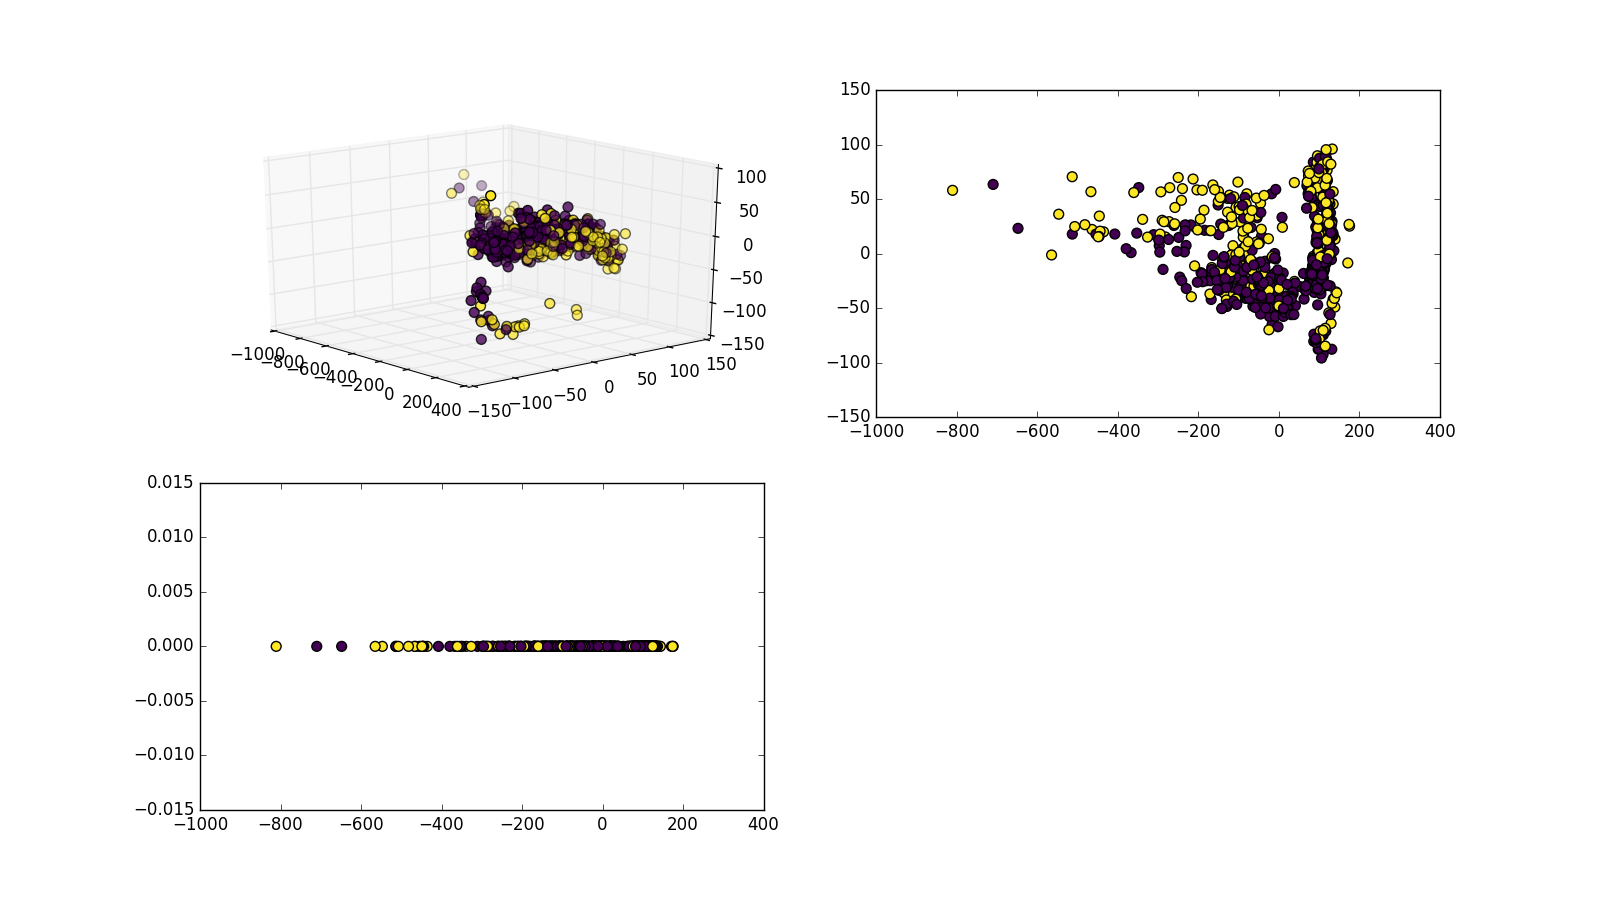
\includegraphics[width=.85\linewidth]{img/experiments/iso_diabetes}
	\captionsetup{justification=centering}
	\caption{The Diabetes data set and its reduction to 3, 2 and 1 dimensions, respectively.}
	\label{fig:iso_diabetes}
\end{figure}

\begin{table}[H]
	\centering
	\begin{tabular}{|c|c|c|c|c|c|}
		\hline
		& \textbf{Orig. ($\mathbb{R}^{8}$}) & \textbf{$\mathbb{R}^{6}$} & \textbf{$\mathbb{R}^{4}$} & \textbf{$\mathbb{R}^{2}$} & \textbf{$\mathbb{R}$} \\\hline
		\textbf{Pred. accuracy}   & .7239 & .7174 & .7252 & .7148 & .6588 \\\hline
		\textbf{GridSearch time}   & .79 s & .94 s & .58 s & .99 s & 7.4 s \\\hline
		\textbf{Reduction time}    & - & 23.55 s & 24.38 s & 26.5 s & 23.44 s \\\hline
		\textbf{Stress} & - & .2875 & .2362 & .3001 & .4462 \\\hline
		\textbf{Data size}  & 48 KB & 36 KB & 24 KB & 12 KB & 6 KB \\\hline
	\end{tabular}
	\captionsetup{justification=centering}
	\caption{Description of predictions and reduction performance for Diabetes data set.}
\end{table}
